\documentclass[12pt]{scrartcl}
\usepackage{config}
\usepackage{minted}

%\newcommand\mrh{\color{white}\bfseries}
\newcommand\mrc[1]{\begin{tabular}{@{}l@{}} #1 \end{tabular}}
\setlength\arrayrulewidth{0.8pt}

\usemintedstyle{pastie}

\begin{document}
    \hh{Determina Aristas}
    
    
    \vspace{10pt}

    
    \hh{Problema}
    
        Te es dado un entero $N$ y $N - 1$ aristas bidireccionales. Estas aristas conectan $N$ vértices de tal forma que exista un camino\footnote{Secuencia de vértices tal que cualesquiera dos adyacentes pertenecen a una arista del grafo.} entre cualesquiera dos vértices (es decir, forman un árbol). Debes especificar pesos para cada una de las aristas, de tal forma que se cumpla la siguiente propiedad en el árbol:
        
        Para cada entero $x$ entre $1$ y $\left\lfloor \frac{2N^2}{9} \right\rfloor$, existe una pareja de vértices $i, j$, tal que la suma de los pesos en el camino simple\footnote{Que no repite aristas.} entre $i$ y $j$ es igual a $x$.
    
    \hh{Detalles de Implementación}

        Debes implementar la función \textit{Determinar\_aristas()}. Esta función recibe un entero $N$ y dos vectores $u$ y $v$, cada uno con $N - 1$ elementos. para cada $0 \le i \le N - 2$, $u[i]$ y $v[i]$ son los vértices que se conectan con la arista $i$. Esta función debe regresar un vector con $N - 1$ arreglos de 3 elementos, los primeros dos elementos de estos arreglos deben contener los vértices de una arista, y el tercero el peso que elegiste. Las aristas en este vector pueden ir en cualquier orden.
        La función se vería así:

\begin{minted}{c++}
#include <bits/stdc++.h>
using namespace std;

vector<array<long long, 3>> Determina_aristas(int N,
    vector<int> u, vector<int> v) {
    // Implementa esta función.
}
\end{minted}

    El evaluador correrá la función \textbf{múltiples} veces por cada caso de prueba.

    \hh{Ejemplo}
    
        {\itshape Ejemplo 1:}
        \begin{itemize}
            \item El evaluador llama la función 
            \begin{center}
                \textit{Determina\_aristas(6, \{0, 1, 2, 2, 1\}, \{1, 2, 3, 4, 5\})}
            \end{center}
            el árbol en este caso es el siguiente:
            \begin{center}
                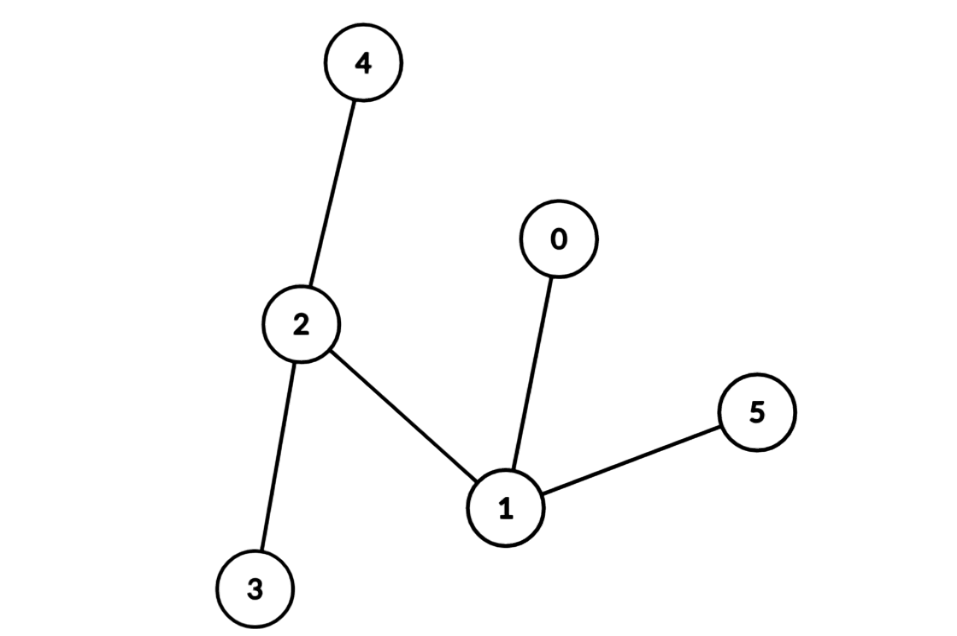
\includegraphics[scale=0.25]{ej1.png}
            \end{center}
            \item Podrías obtener la totalidad de los puntos que represente este caso respondiendo el vector \{\{0, 1, 2\}, \{1, 2, 1\}, \{5, 1, 5\}, \{2, 3, 2\}, \{2, 4, 4\} \}. Que corresponde a la siguiente elección de aristas:
            \begin{center}
                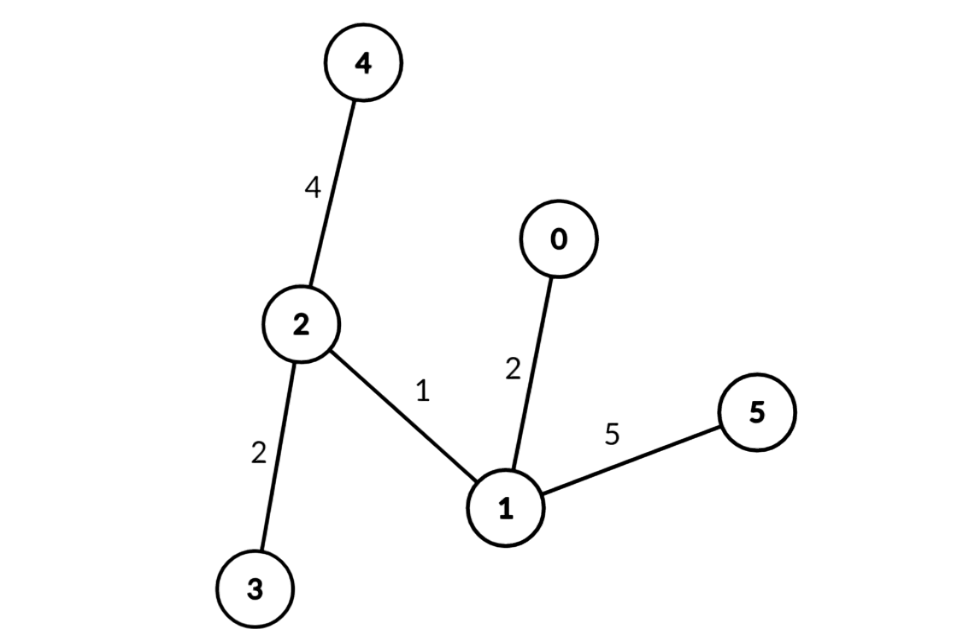
\includegraphics[scale=0.25]{ej2.png}
            \end{center}
            Esto es porque:
            \begin{itemize}
                \item El camino entre los vértices $(1, 2)$ tiene peso 1.
                \item El camino entre los vértices $(0, 1)$ tiene peso 2.
                \item El camino entre los vértices $(0, 2)$ tiene peso 3.
                \item El camino entre los vértices $(2, 4)$ tiene peso 4.
                \item El camino entre los vértices $(1, 5)$ tiene peso 5.
                \item El camino entre los vértices $(2, 5)$ tiene peso 6.
                \item El camino entre los vértices $(0, 5)$ tiene peso 7.
                \item El camino entre los vértices $(3, 5)$ tiene peso 8.
            \end{itemize}
        \end{itemize}
        k

    \hh{Consideraciones}
        \begin{itemize}
            \item $4 \le N \le 2000$.
            \item Los vectores $u$ y $v$ tendrán exactamente $N - 1$ elementos.
            \item Para cada $0 \le i \le N - 2$, se cumple que $0 \le u[i] \neq v[i] \le N - 1$. 
            \item Se garantiza que el grafo formado por las aristas es un árbol.
            \item sea $S_N$ la suma de los valores de $N$ sobre todas las llamadas a la función en un caso. Se cumple que $S_N \le 2000$.
        \end{itemize}
    
    \hh{Subtareas}


    \begin{itemize}
        \item (3 puntos) $N \le 4$.
        \item (7 puntos) Obtendrás los puntos de esta subtarea si tu elección de aristas cumple con la condición para $1 \le x \le N$.
        \item (11 puntos) Para todo $0 \le i \le N - 1$  se cumple que la cantidad de aristas que tienen a $i$ como vértice es $1$ o $N - 1$.
        \item (21 puntos) Para todo $0 \le i \le N - 2$, se cumple que $u[i] = i + 1, v[i] = i$.
        \item (21 puntos) Para todo $0 \le i \le N - 2$, se cumple que $u[i] = i + 1, v[i] = \left\lfloor\frac{i}{2} \right\rfloor$.
        \item (37 puntos) Sin restricciones adicionales.
    \end{itemize}
\end{document}
